\clearpage
\pagenumbering{arabic}
\setcounter{page}{1}

\phantomsection
\label{ch:intro}
\chapter{Introduction}

% This chapter presents about what is OCR? why it is needed, and
% what are the challenges in OCR. It also presents the problem 
% for OCR on Khmer script (non-latin based), and OCR on multilingual
% language such as Khmer and English. We will talk about the scope
% of this research because it'll help us to keep 
% our research scope ensures clarity, direction, and feasibility 
% throughout the study.
\vspace{-1cm}
\setlength{\parindent}{0pt}
\vspace{0.3cm}

\section{Background to the Study}
\label{sec:background}

{\englishfont\fontsize{13.5pt}{17pt}\selectfont OCR technology has revolutionized how we convert printed 
documents into digital text. With recent AI breakthroughs, 
OCR systems now use deep learning to automatically find and 
recognize characters in images. This technology is everywhere from digital libraries to search engines to language translation tools.
For popular languages like English, Chinese, and Japanese, 
OCR works incredibly well. These languages have massive 
amounts of training data and researchers have studied 
their text patterns for decades. However, when it comes to 
complex scripts like Khmer, OCR technology is still way behind.
Cambodia is in desperate need of better OCR right now. 
The country has been rapidly digitizing over the last 
two decades. Everyone wants to convert Khmer documents such as
textbooks, historical records, cultural materials 
into digital formats for education and research.
There's a huge problem with Khmer script which is extremely complicated.
English letters just line up in 
a row from left to right while Khmer characters pile on top 
of each other in complex ways. They have tiny accent 
marks, subscripts, and vowel symbols that can appear 
above, below, or wrapped around the main letter. If 
there is missing even a small mark, the word meaning 
is completely changed.

\begin{table}[H]
    \centering
    \caption{Why Khmer OCR Is Desperately Needed}
    \vspace{6pt}
    \phantomsection
    \label{sec:textbook}
    \renewcommand{\arraystretch}{1.5} % adjust row height multiplier
    \resizebox{\textwidth}{!}{%
      \begin{tabular}{|p{2.7cm}|p{4.8cm}|p{7cm}|}
        \hline
        \rule{0pt}{0.4cm}\textbf{Sector} & \textbf{Cause} & \textbf{Effect} \\
        \hline
        \rule{0pt}{0.4cm}Education & Physical textbooks & Students cannot search or edit content \\
        \hline
        \rule{0pt}{0.4cm}Libraries & Books rotting on shelves & Knowledge becomes inaccessible \\
        \hline
        \rule{0pt}{0.4cm}Government & Traditional paperwork & Slow bureaucracy, and hard to find \\
        \hline
        \rule{0pt}{0.4cm}Administrative & Handwritten documents & Manual data entry required \\
        \hline
        \rule{0pt}{0.4cm}Culture & Ancient texts deteriorating & Loss of heritage records \\
        \hline
      \end{tabular}%
    }
  \end{table}



\section{Problem Statement}
\label{sec:problem}

To develop high accuracy OCR model needs tons of millions 
annotated images. Khmer language resources are extremely 
limited, with only a few thousand quality annotated samples 
available. Moreover, as mentioned from previous section 
Khmer scripts is very complicated \citep{Huffman1987cambodian}.   Characters stack on 
top of each other with just tiny changes in the script 
marks could differentiate the word meaning. There are 
multiple problems with Khmer writing system that make it 
difficult to implement OCR model as listed below:

\begin{enumerate}
    \item \textbf{Complex Character Structure:} Khmer script presents unique recognition challenges due to its intricate character composition. Unlike Latin scripts, Khmer characters feature complex stacking arrangements with diacritics, subscripts, and vowel markers positioned above, below, or surrounding base characters. Even minor mark omissions can drastically alter word meanings, making precise recognition critical.
    
        \begin{figure}[H]
            \centering
            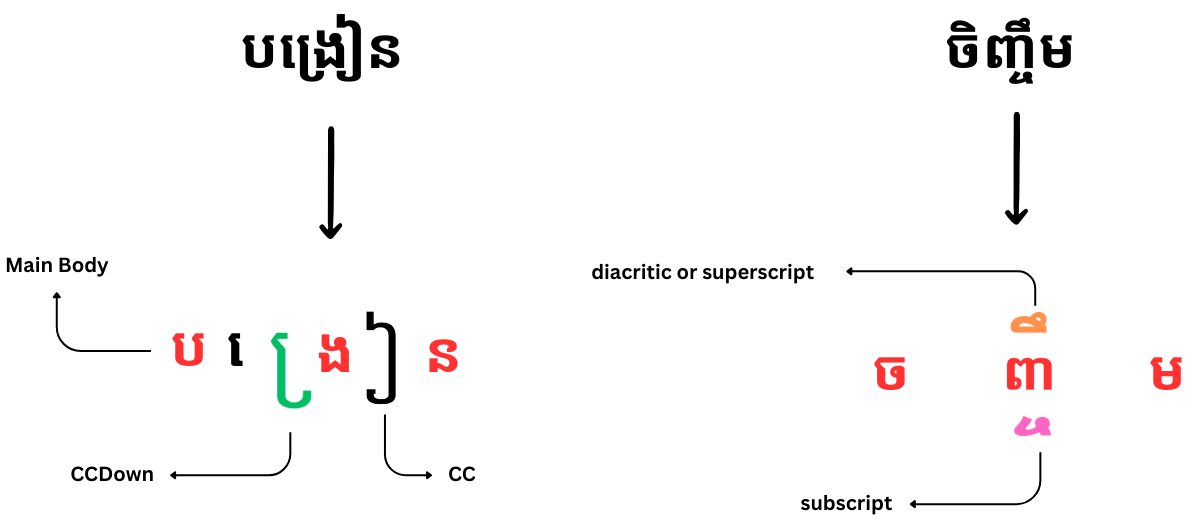
\includegraphics[width=0.87\textwidth]{figures/example_of_text_format.png}
            \begin{minipage}{0.87\textwidth}
                \caption{Example of Khmer text format showing the complexity of character combinations and diacritics \citep{Buoy2022}}.
                \label{fig:text_format}
            \end{minipage}
        \end{figure}
 
    \item \textbf{Inconsistent Word Boundaries:} Khmer lacks standardized word spacing conventions, creating significant segmentation challenges. While English consistently uses spaces between words, Khmer writers apply spacing inconsistently or omit it entirely. This variability makes it extremely difficult for OCR systems to determine word boundaries accurately.
    
        \begin{figure}[H]
            \centering
            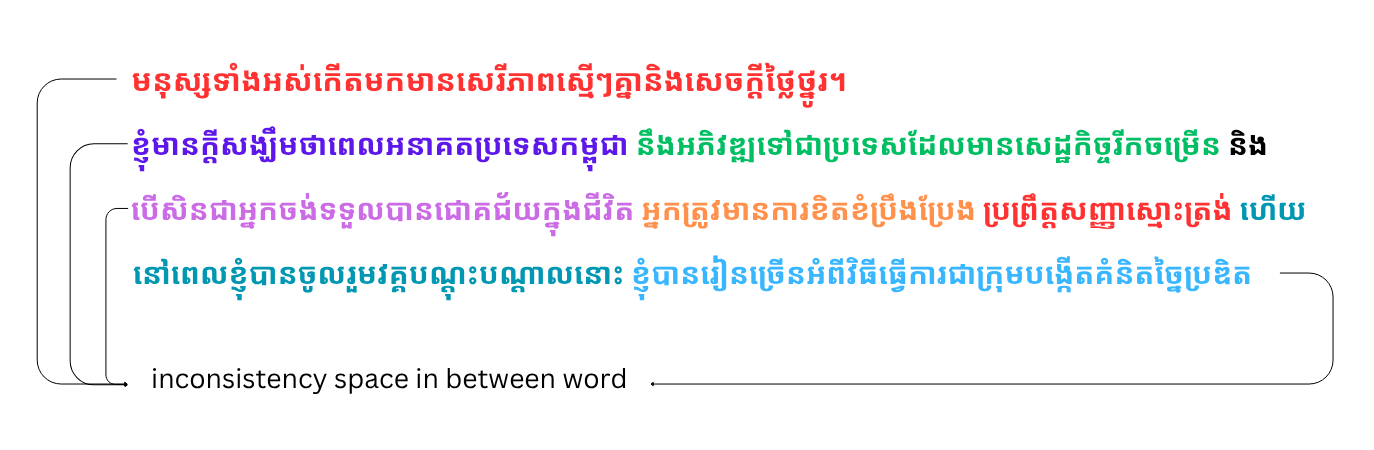
\includegraphics[width=0.87\textwidth]{figures/example_of_long_text.png}
            \begin{minipage}{0.87\textwidth}
                \caption{Example of sequential Khmer text showing how characters combine to form syllables and words}
                \label{fig:sequential_text}
            \end{minipage}
        \end{figure}
 
    \item \textbf{Mixed-Language Complexity:} Cambodia's increased English education and international business integration over recent decades has led to widespread mixed-language documents. Signs, textbooks, and digital content frequently blend Khmer and English within single sentences or paragraphs, creating OCR challenges including script transition confusion, conflicting layout patterns, and font inconsistencies \citep{Wilwohl}.
    
        \begin{figure}[H]
            \centering
            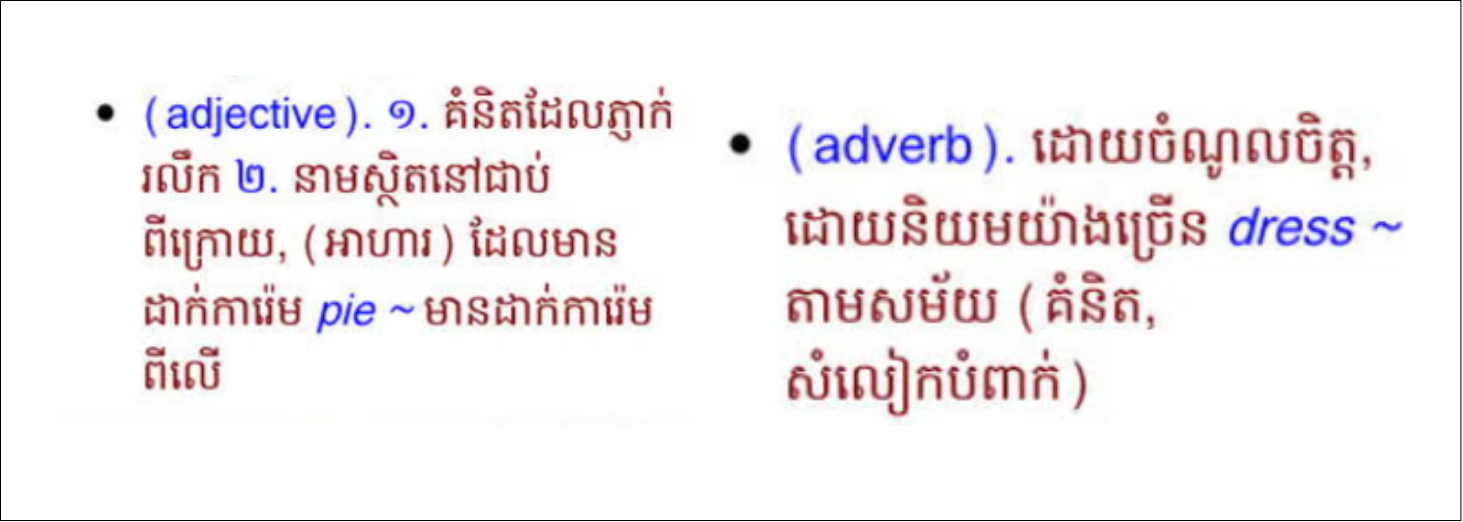
\includegraphics[width=0.87\textwidth]{figures/mix_language_khmer_and_english.png}
            \begin{minipage}{0.87\textwidth}
                \caption{Example of mixed Khmer-English text showing how both languages appear together in modern Cambodian documents}
                \label{fig:mix_language}
            \end{minipage}
        \end{figure}
        
        Current Khmer OCR systems typically target single-language scenarios and struggle with mixed-language content prevalent in modern Cambodia. The scarcity of properly annotated multilingual datasets compounds this challenge, limiting model training effectiveness and recognition accuracy.
 
    \item \textbf{Font Variation Challenges:} While English utilizes approximately 15-25 common fonts according to industry studies from rigorousthemes.com, lifehack.org, and indeed.com, Khmer encompasses numerous visually distinct font families ranging from bold and thick to thin and decorative styles. Models trained on limited font sets often fail when encountering different typefaces, highlighting the need for comprehensive font coverage in training data.
    
        \begin{figure}[H]
            \centering
            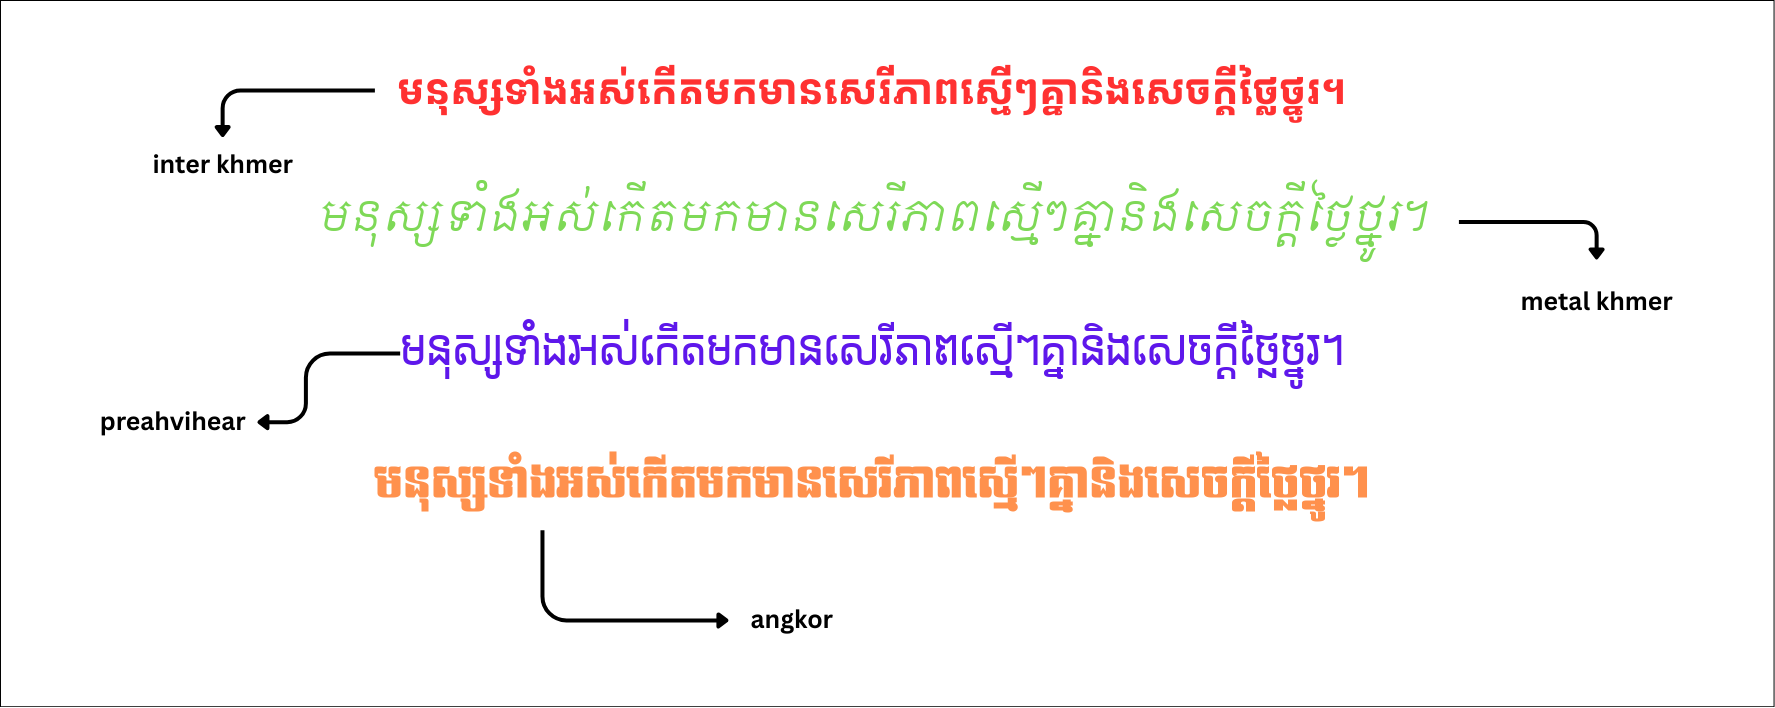
\includegraphics[width=0.87\textwidth]{figures/varianty_of_font.png}
            \begin{minipage}{0.87\textwidth}
                \caption{Examples of the same Khmer text rendered in different fonts, demonstrating the significant visual variations that OCR systems must handle}
                \label{fig:font_variants}
            \end{minipage}
        \end{figure}
 
    \item \textbf{Character Stacking Patterns:} Khmer employs sophisticated vertical and horizontal character stacking to form syllables and words, creating complex spatial relationships that challenge traditional OCR architectures. These multidimensional arrangements require specialized recognition approaches capable of understanding hierarchical character dependencies.
    
        \begin{figure}[H]
            \centering
            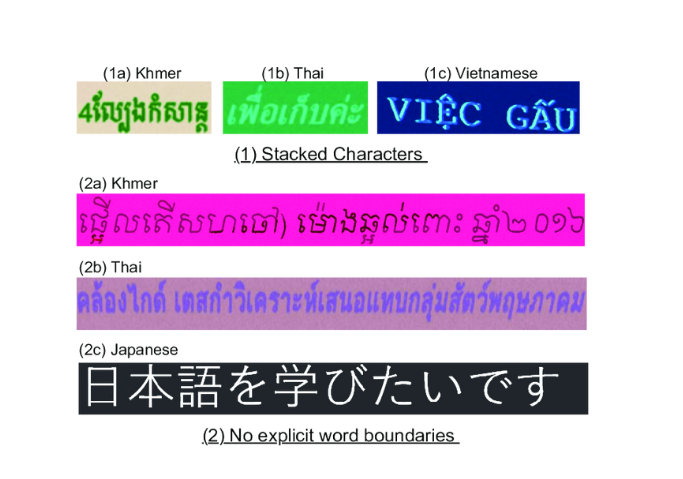
\includegraphics[width=0.87\textwidth]{figures/text_stacking_mixing_language.png}
            \begin{minipage}{0.87\textwidth}
                \caption{Illustration of Khmer text stacking patterns, showing how characters combine vertically and horizontally to form syllables and words \citep{buoy2023khmerocr}}
                \label{fig:text_stacking}
            \end{minipage}
        \end{figure}

        \item \textbf{Ambiguity in Khmer Character Rendering:} Certain Khmer characters, especially subscript forms like subscript DA and subscript TA, can appear visually identical despite having different Unicode encodings. This leads to high intra-class variance and low inter-class variance, making OCR difficult. As shown in Fig.~\ref{fig:khmer_text_ambiguous}, different char but hard to recognize between characters, increasing recognition errors.
        \begin{figure}[H]
            \centering
            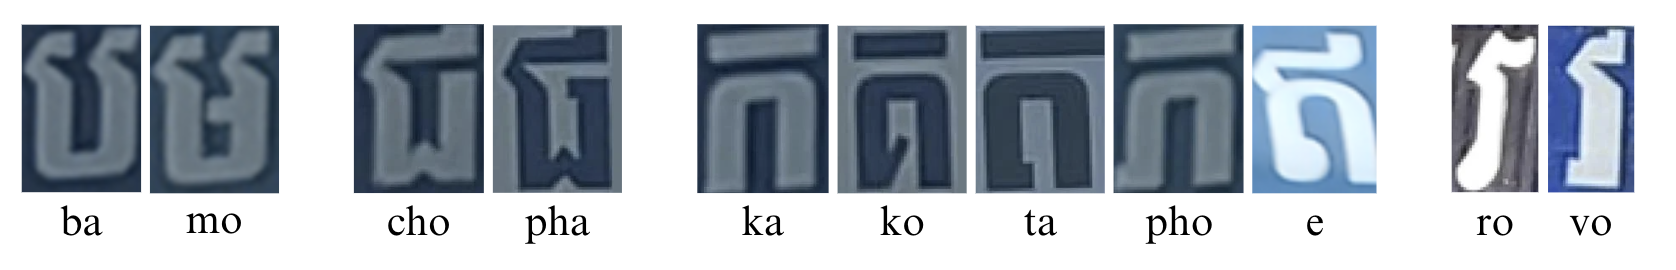
\includegraphics[width=0.87\textwidth]{figures/ambiguous_problem.png}
            \begin{minipage}{0.87\textwidth}
                \caption{Same characters having ambiguous text render \citep{nom2024khmerst}}
                \label{fig:khmer_text_ambiguous}
            \end{minipage}
        \end{figure}
 \end{enumerate}


\section{Aim and Objectives of the Study}
\label{sec:objectives}

Our main goal is to create high performance OCR system 
that can handle mixed writing language of Khmer and 
English in the same document. Our objectives mainly are:

\begin{enumerate}
    \item \textbf{Create a text annotation tool:} Build a tool that can efficiently mark up images with bounding boxes and text labels for both text detection and recognition tasks.

    \item \textbf{Generate synthetic data that actually helps:} To collect real data is expensive and time-consuming, we create millions of synthetic images with different fonts, backgrounds, and realistic distortions that look authentic enough to train the models effectively.

    \item \textbf{Build an end-to-end OCR pipeline:} Customize CRAFT for text detection and TrOCR for recognition, specifically for Khmer script and mixed-language document.

    \item \textbf{Improve over existing solutions:} Aim to achieve better performance and reliable across diverse samples than previous research works or OCR tools such as Tesseract.
    
    \item \textbf{Provide an easy-to-use model:} Deploy our result allowing enthusiast individual easily accessible to experiment with minimal setup. This approach hope to expand the application of OCR in Khmer language.
\end{enumerate}


\section{Rationale of the Study}
\label{sec:rationale}
       This research is motivated by several compelling factors. First, there is an urgent need to digitize and preserve Cambodia's vast textual heritage, including historical documents, educational materials, and cultural artifacts. Without effective OCR technology for Khmer script, this digitization process remains labor-intensive and prone to errors.
       Second, the current limitations of OCR systems for Khmer significantly hinder educational and academic initiatives in Cambodia. Many educational institutions struggle to convert physical textbooks and learning materials into digital formats, impacting accessibility and modernization efforts in education.
       Third, the unique challenges posed by Khmer script from character stacking to the absence of word boundaries present an opportunity to advance the field of OCR technology as a whole. Solutions developed for Khmer may benefit other scripts with similar characteristics.
       Finally, improving Khmer OCR technology aligns with broader digital transformation goals in Cambodia, supporting efforts to preserve cultural heritage while enabling more efficient information processing and accessibility in various sectors.

\section{Limitations and Scope}
\label{sec:limitations}

While this research aims to advance Khmer OCR technology significantly, it is important to acknowledge certain limitations and define the scope of the study:

\begin{enumerate}
    \item The research focuses specifically on printed text of Khmer and English and does not address handwritten in text recognition context, which presents additional challenges requiring further development.
    
    \item The study primarily considers modern Khmer fonts and typography, with limited coverage of historical or decorative text styles.
    
    \item While the system aims to handle various levels of document quality, the extremely degraded or damaged documents may fall outside the scope of reliable recognition.
    
    \item The study focuses on optical character recognition and does not extend to higher-level natural language processing tasks such as semantic analysis or machine translation.
    
    \item Resource constraints may limit the size and diversity of the training dataset, further efforts will be made to ensure sufficient representation of common use cases.
\end{enumerate}

These limitations help maintain a focused research scope while acknowledging areas that may require future investigation.

\section{Structure of the Thesis}
\label{sec:structure}

This thesis is structured into the following chapters:

\begin{enumerate}
   \item \textbf{Introduction}: Establishes the research context, defines objectives, outlines key research questions, explains the study's importance, and sets clear boundaries for the investigation.
   
   \item \textbf{Literature Review}: Examines current OCR technologies, identifies specific challenges in Khmer script processing, and explores relevant deep learning methodologies.
   
   \item \textbf{Dataset Construction}: Describes our data collection process, synthetic data generation techniques, preprocessing methods, and dataset quality evaluation.
   
   \item \textbf{Model Architecture and Experiments}: Details our proposed OCR pipeline, explains model customizations for Khmer script, and outlines training methodologies.
   
   \item \textbf{Results and Analysis}: Reports experimental findings, analyzes performance metrics, and compares our system against existing OCR solutions.
   
   \item \textbf{Discussion and Future Work}: Interprets results, discusses limitations, and identifies opportunities for future research and improvements.
   
   \item \textbf{Conclusion}: Synthesizes key contributions, summarizes main findings, and highlights the broader impact on Khmer OCR development.
\end{enumerate}

Each chapter progressively builds on previous sections to deliver a complete investigation of advanced Khmer OCR technology development.

}